\setcounter{secnumdepth}{5}

\chapter{Scanning - realizzazione in python}
La prima fase dell'attacco portato a compimento è la fase di scanning. In questa fase ci si è occupati della creazione di uno script python che si presenta, all'avvio, in questo modo:

\begin{figure}[H]
    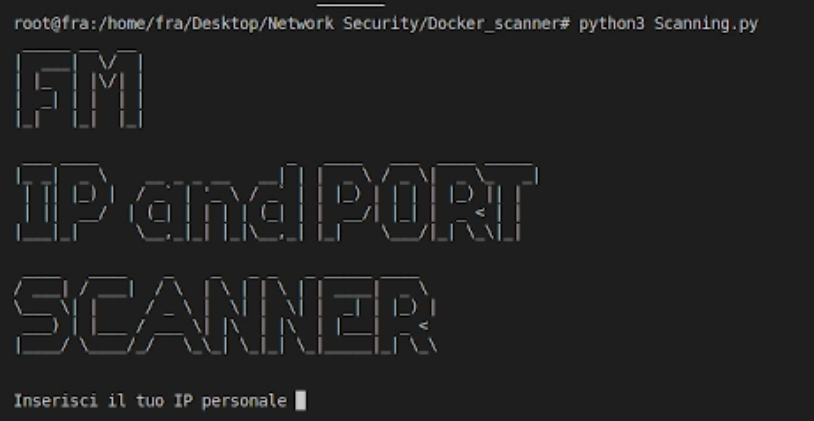
\includegraphics[scale=0.5]{UNINA_MSc_Thesis_Project/img/Esecuzione/Scanning_start.png}
    \centering
    \caption{Start}
    \label{fig:my_label}
\end{figure}

La prima richiesta è quella di inserimento dell'IP personale: questo è utile in quanto, una volta inserito l'IP, permette di ricercare tutti gli IP vivi all'interno di quella sottorete (considerata una subnet mask 255.255.255.0). 

Successivamente, viene generato un file \textbf{\textit{IPalive.txt}} che contiene, al suo interno, tutti gli IP "vivi" in rete. 

\begin{figure}[H]
    \centering
    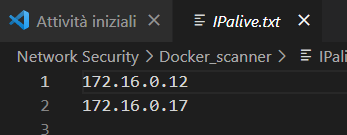
\includegraphics{UNINA_MSc_Thesis_Project/img/Esecuzione/ipalive.png}
    \caption{IPalive.txt}
    \label{fig:my_label}
\end{figure}

Successivamente, viene chiesto quale tipo di scanning effettuare:

\begin{figure}[H]
    \centering
    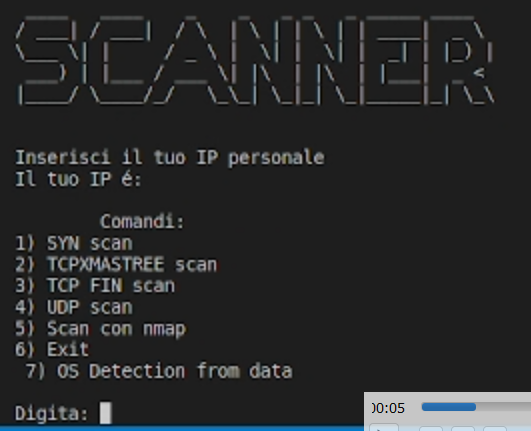
\includegraphics[scale=0.6]{UNINA_MSc_Thesis_Project/img/Esecuzione/ScanningChoice.png}
    \caption{Scelta dello scanning}
    \label{fig:my_label}
\end{figure}
Al termine, si ottengono i file: "SynScan.txt", "TCPFinScan.txt", etc.. a seconda del tipo di scan scelto. Questo si presenterà con la dicitura $IP-portaAperta$:

\begin{figure}[H]
    \centering
    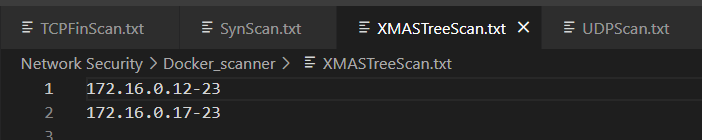
\includegraphics[scale=0.8]{UNINA_MSc_Thesis_Project/img/Esecuzione/scannerResults.png}
    \caption{Risultati dello scanning: porta 23 aperta nei due bots}
    \label{fig:my_label}
\end{figure}
% \lipsum[1][1-3]

Selezionando scan con nmap, viene fatto uso delle librerie python-nmap che scansionano le porte dalla 1 alla 2323 e dà, in output, un file contenente:
\begin{itemize}
    \item Porte aperte (+ servizio aperto)
    \item Sistema Operativo in utilizzo sull'IP
    \item ..altre informazioni
\end{itemize}

\begin{figure}[H]
    \centering
    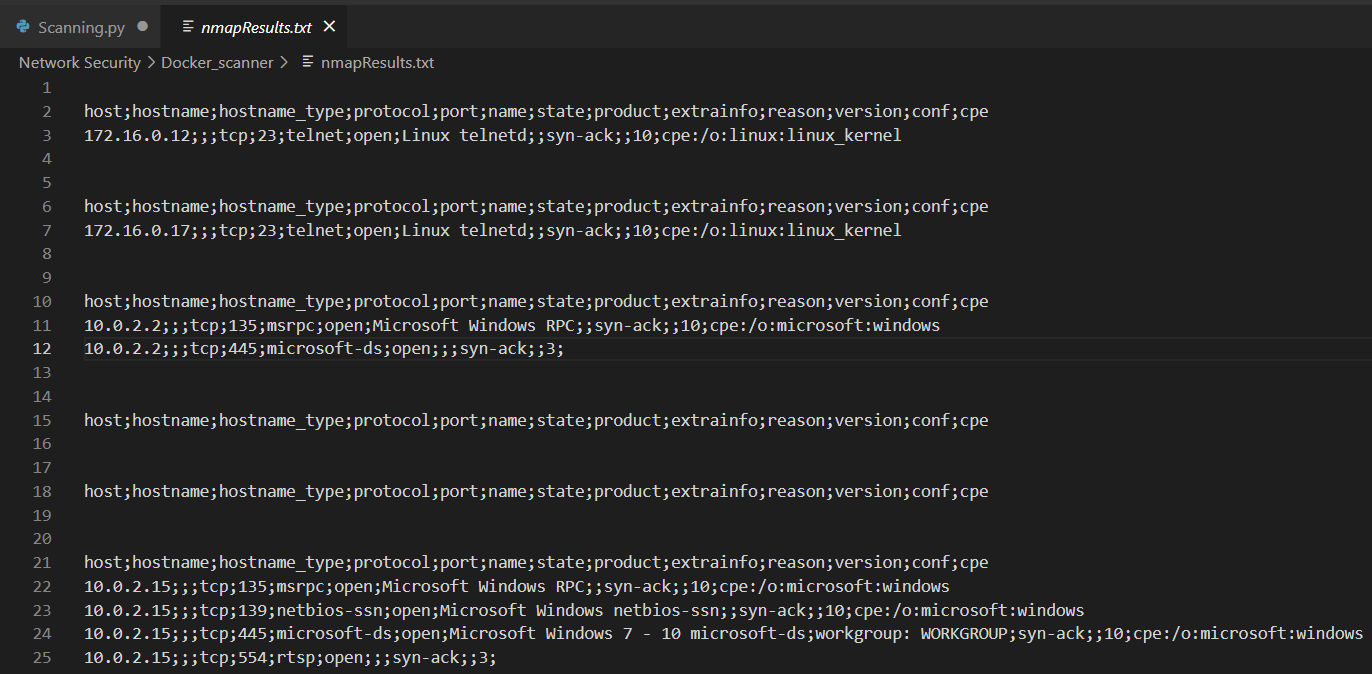
\includegraphics[scale=0.4]{UNINA_MSc_Thesis_Project/img/nmapResult.png}
    \caption{Risultati dello scanning: porta 23 aperta nei due bots}
    \label{fig:my_label}
\end{figure}

Selezionando "OS Detection" viene effettuata una detection del sistema operativo, andando ad aprire uno dei file output dello scanning e andando a verificare le porte aperte dei singoli nodi. 
Ad esempio:
\begin{itemize}
    \item Porte aperte: 135 (endpoint mapper), 139 (NetBIOS), 445 (Active Directory) \xrightarrow[]{}Windows$
    
    \item Porte aperte: 22 (SSH), 111 (SUN RPC), 2049 (NFS) \xrightarrow[]{}Linux$
    
\end{itemize}


Terminato lo scanning, digitando 6, si esce dalla fase di scanning per passare alla fase di \textbf{creazione della botnet}. 

\section{Codice}
La funzione che cerca nodi attivi all'interno della rete è la seguente. Essa procede ad una ricerca all'interno della rete facendo uso del comando "ping" di (iputils-ping) con un timeout di 2 secondi. Il sistema invia più richieste Echo ICMP (Internet Control Message Protocol - che si occupa di trasmettere informazioni riguardanti malfunzionamenti, informazioni di controllo) all'indirizzo IP o all'URL del sistema remoto. Se la risposta arriva, allora il nodo è attivo; viceversa, il nodo è spento.
\begin{figure}[H]
    \centering
    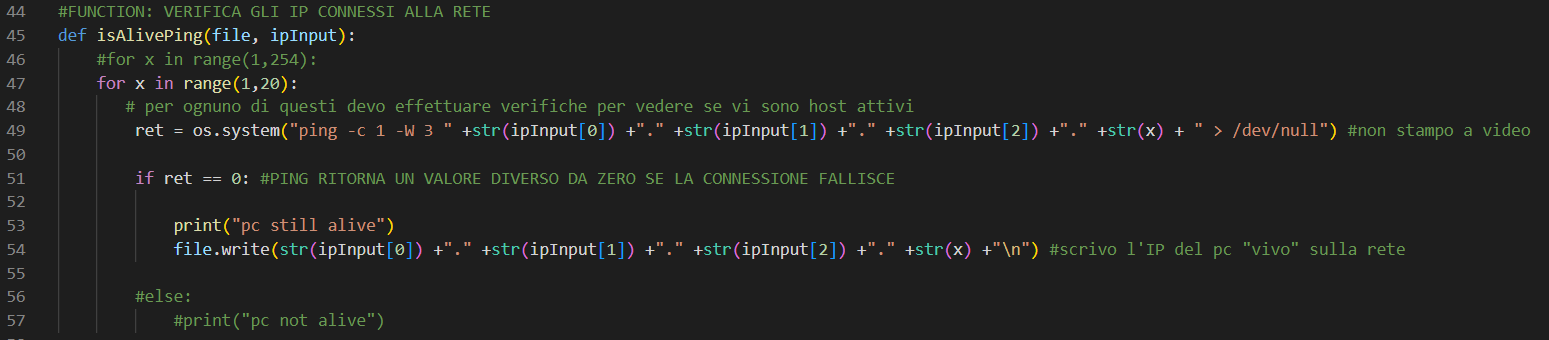
\includegraphics[scale=0.4]{UNINA_MSc_Thesis_Project/img/Codice/isAlive.png}
    \caption{isAlive}
    \label{fig:my_label}
\end{figure}

Per la chiusura delle connessioni mezze aperte (Handshake non terminato) viene usato la seguente funzione di reset che invia i flag $ACK=RESET=1$ su TCP
\begin{figure}[H]
    \centering
    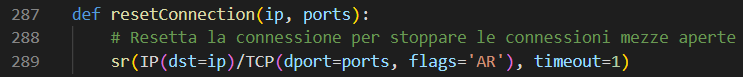
\includegraphics[scale=0.7]{UNINA_MSc_Thesis_Project/img/Codice/resetConnection.png}
    \caption{resetConnection}
    \label{fig:my_label}
\end{figure}

Funzione SYN SCAN: creazione del pacchetto con il flag syn alto e in attesa di ricevere, se la porta è aperta, di SYN/ACK.
\begin{figure}[H]
    \centering
    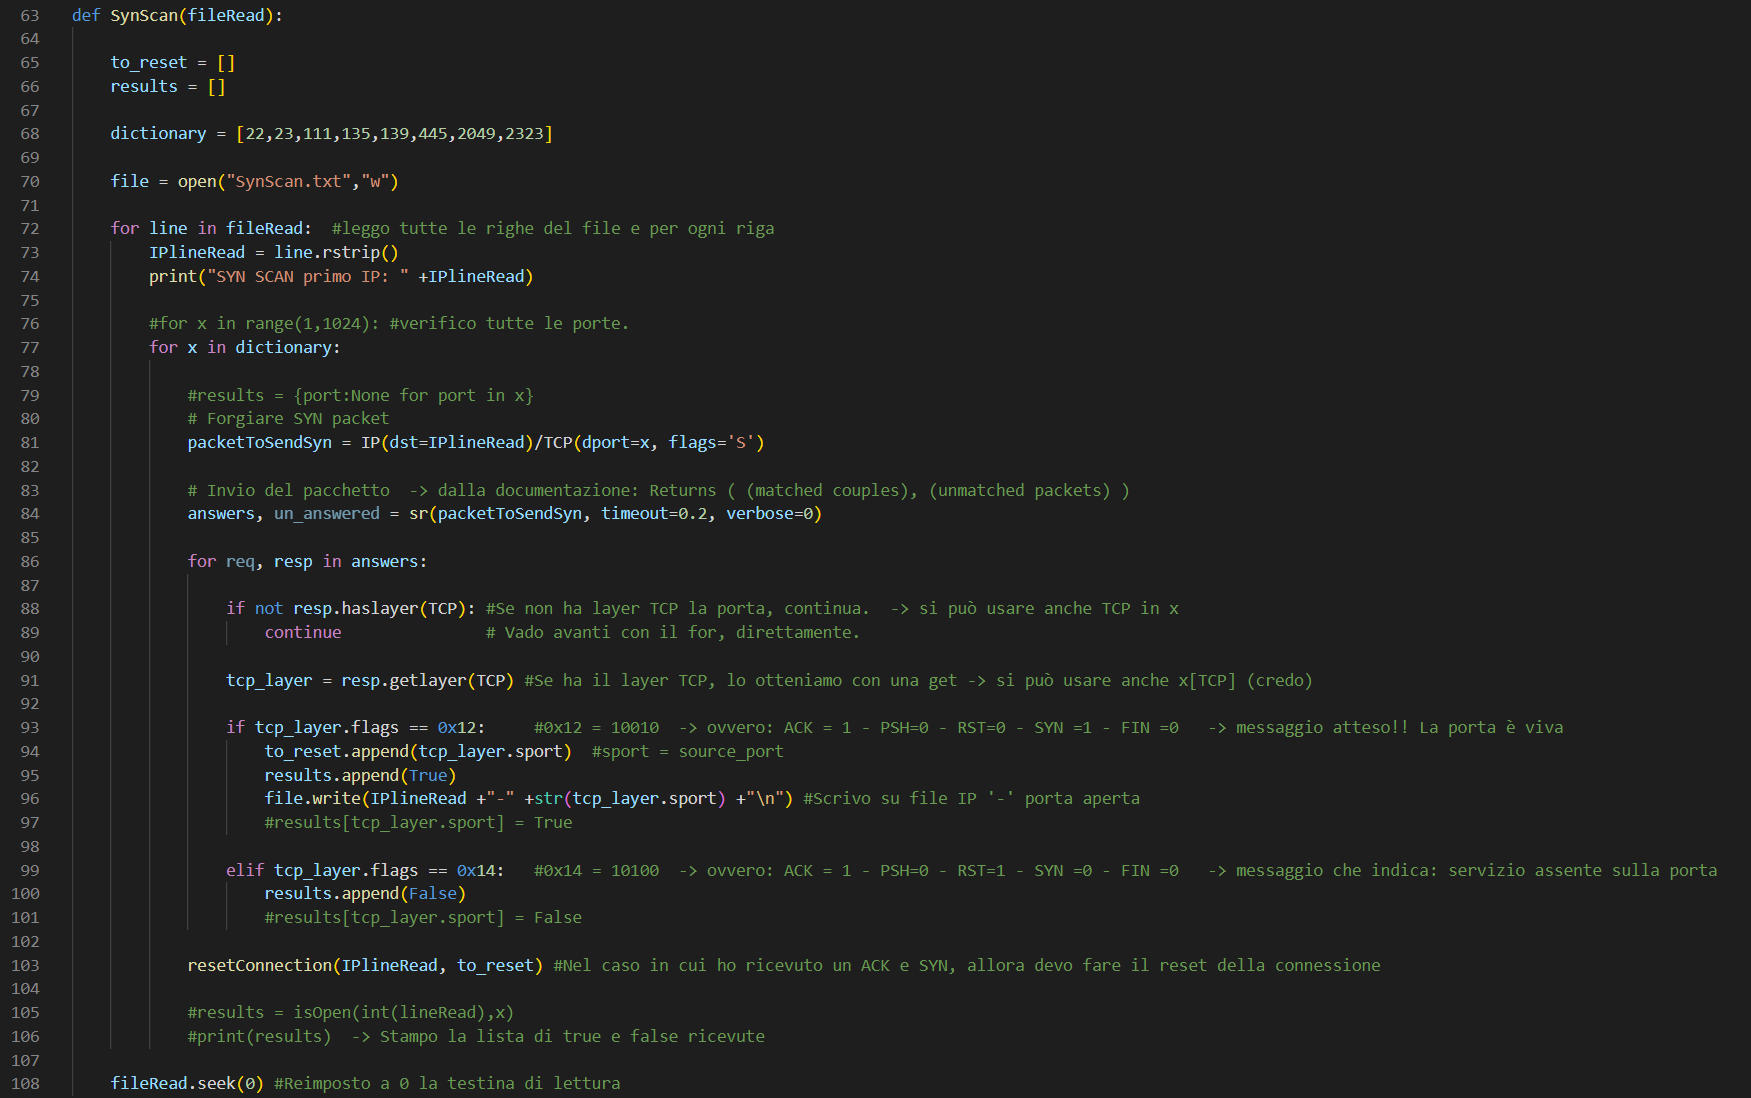
\includegraphics[scale=0.3]{UNINA_MSc_Thesis_Project/img/Codice/SynScan.png}
    \caption{SYN scan}
    \label{fig:my_label}
\end{figure}

Il XMASTree, così come il FIN scan ($FIN=1$), invia un messaggio con i flag $URG=FIN=PSH=1$ (da qui il nome "Albero di natale"). Se non arriva nessuna risposta, allora il nodo è attivo, viceversa, viene ricevuto un pacchetto con flag $RST=1$

\begin{figure}[H]
    \centering
    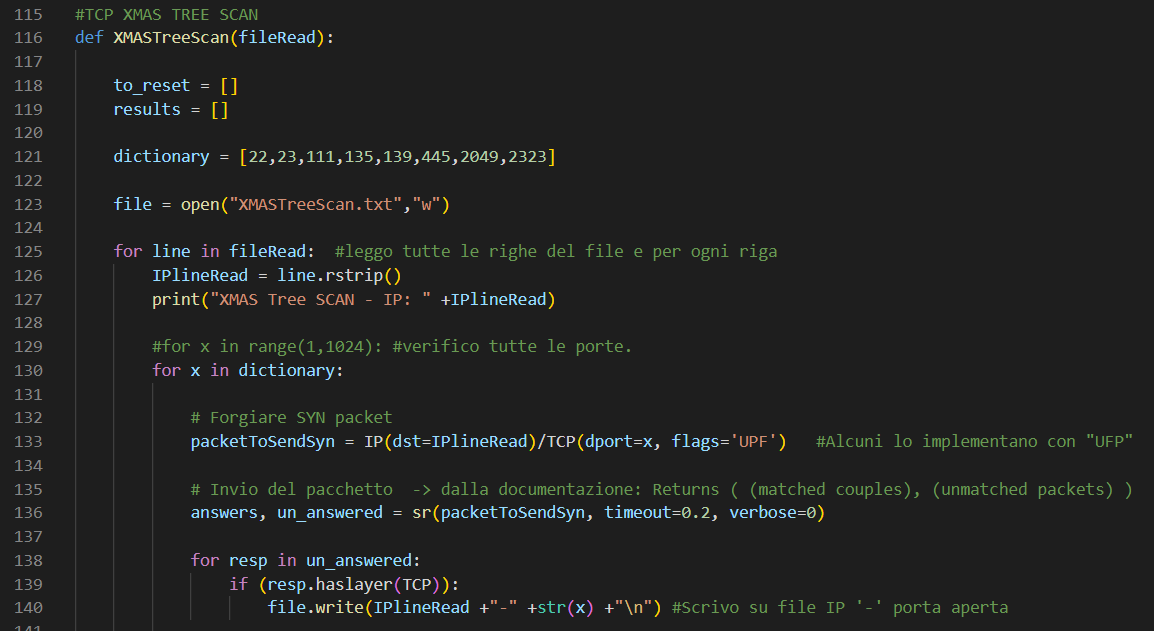
\includegraphics[scale=0.4]{UNINA_MSc_Thesis_Project/img/Codice/XMASTree.png}
    \caption{XMASTree Scan}
    \label{fig:my_label}
\end{figure}

Funzione per UDP scan: essa controlla se il pacchetto UDP ricevuto ha come risposta:
\begin{itemize}
    \item Porta chiusa: un pacchetto ICMP tipo 3, codice 3
    \item Pacchetto fIltrato: pacchetto ICMP tipo 3, codice 1,2,9,10,13
    \item Porta aperta: altri casi. In particolare, viene controllato se la risposta ha il "\textit{layer UDP}".
\end{itemize}

\begin{figure}[H]
    \centering
    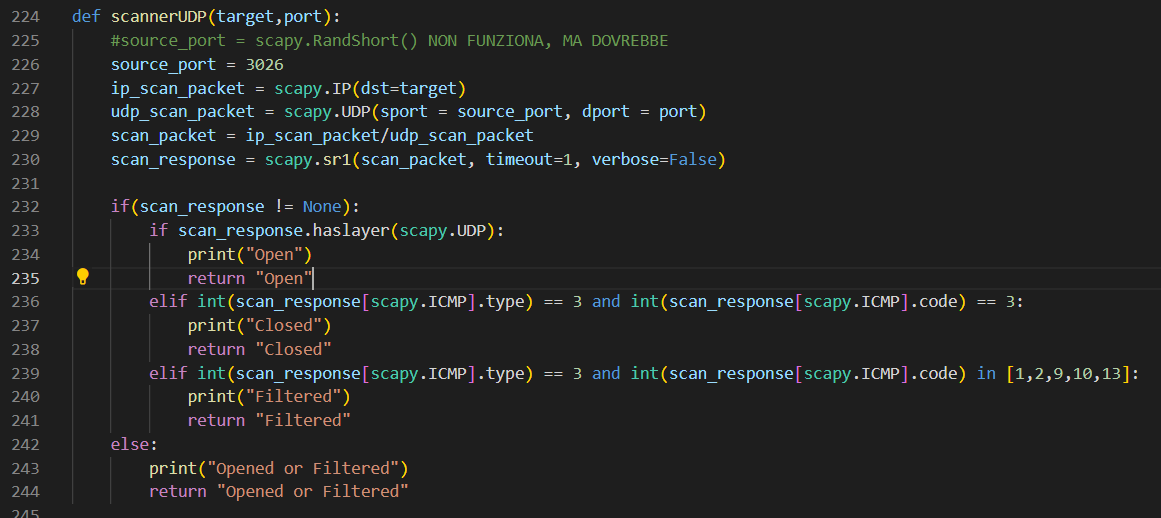
\includegraphics[scale=0.4]{UNINA_MSc_Thesis_Project/img/Codice/UDPScanner.png}
    \caption{UDP Scan}
    \label{fig:my_label}
\end{figure}

Funzione di Scan attraverso la libreria nmap con la funzione $nmap.PortScanner()$:

\begin{figure}[H]
    \centering
    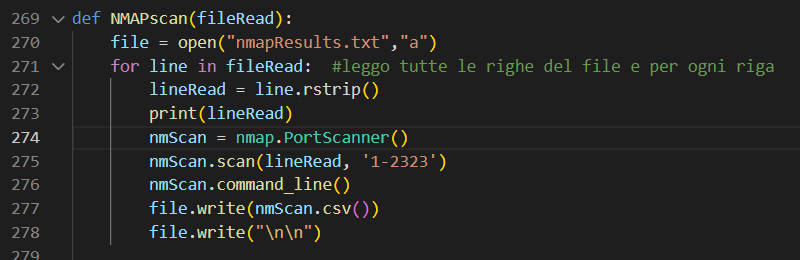
\includegraphics[scale=0.5]{UNINA_MSc_Thesis_Project/img/Codice/nmapScan.png}
    \caption{nmapScan}
    \label{fig:my_label}
\end{figure}


% \lipsum



